


\tikzset{every picture/.style={line width=0.75pt}} %set default line width to 0.75pt        

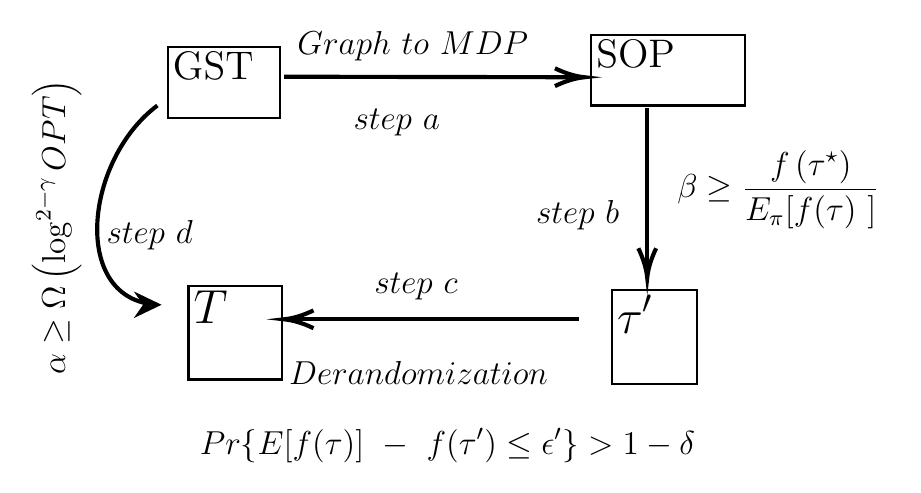
\begin{tikzpicture}[x=0.75pt,y=0.75pt,yscale=-1,xscale=1]
%uncomment if require: \path (0,621); %set diagram left start at 0, and has height of 621

%Straight Lines [id:da2120545823988531] 
\draw [line width=1.5]    (303,411.13) -- (444.75,411.37) ;
\draw [shift={(447.75,411.38)}, rotate = 180.1] [color={rgb, 255:red, 0; green, 0; blue, 0 }  ][line width=1.5]    (14.21,-4.28) .. controls (9.04,-1.82) and (4.3,-0.39) .. (0,0) .. controls (4.3,0.39) and (9.04,1.82) .. (14.21,4.28)   ;
%Straight Lines [id:da8426033767275076] 
\draw [line width=1.5]    (445,528) -- (306,528) ;
\draw [shift={(303,528)}, rotate = 360] [color={rgb, 255:red, 0; green, 0; blue, 0 }  ][line width=1.5]    (14.21,-4.28) .. controls (9.04,-1.82) and (4.3,-0.39) .. (0,0) .. controls (4.3,0.39) and (9.04,1.82) .. (14.21,4.28)   ;
%Straight Lines [id:da17896876306163279] 
\draw [line width=1.5]    (478,426.13) -- (478,505) ;
\draw [shift={(478,508)}, rotate = 270] [color={rgb, 255:red, 0; green, 0; blue, 0 }  ][line width=1.5]    (14.21,-4.28) .. controls (9.04,-1.82) and (4.3,-0.39) .. (0,0) .. controls (4.3,0.39) and (9.04,1.82) .. (14.21,4.28)   ;
%Curve Lines [id:da9340908620330151] 
\draw [line width=1.5]    (242,425) .. controls (207.08,451.19) and (200.39,516.9) .. (240.17,520.82) ;
\draw [shift={(244,521)}, rotate = 180] [fill={rgb, 255:red, 0; green, 0; blue, 0 }  ][line width=0.08]  [draw opacity=0] (13.4,-6.43) -- (0,0) -- (13.4,6.44) -- (8.9,0) -- cycle    ;

% Text Node
\draw    (247,397) -- (301,397) -- (301,431) -- (247,431) -- cycle  ;
\draw (248,398) node [anchor=north west][inner sep=0.75pt]  [font=\Large] [align=left] {GST};
% Text Node
\draw    (451,391) -- (525,391) -- (525,425) -- (451,425) -- cycle  ;
\draw (452,392) node [anchor=north west][inner sep=0.75pt]  [font=\Large] [align=left] {SOP};
% Text Node
\draw    (461,514) -- (502,514) -- (502,559) -- (461,559) -- cycle  ;
\draw (462,515) node [anchor=north west][inner sep=0.75pt]  [font=\LARGE] [align=left] {$\displaystyle \tau ' $};
% Text Node
\draw    (257,512) -- (302,512) -- (302,557) -- (257,557) -- cycle  ;
\draw (258,513) node [anchor=north west][inner sep=0.75pt]  [font=\LARGE] [align=left] {$\displaystyle T$};
% Text Node
\draw (491,445) node [anchor=north west][inner sep=0.75pt]  [font=\large] [align=left] {$\displaystyle \beta \geq \frac{f\left( \tau ^{\star }\right)}{\mathbb{E}_{\pi }[ f( \tau ) \ ]} \ $};
% Text Node
\draw (261,579) node [anchor=north west][inner sep=0.75pt]  [font=\large] [align=left] {$\displaystyle Pr\{\mathbb{E}[ f( \tau )] \ -\ f( \tau ') \leq \epsilon' \}  >1-\delta $};
% Text Node
\draw (308,388) node [anchor=north west][inner sep=0.75pt]  [font=\large] [align=left] {$\displaystyle Graph\ to\ MDP$};
% Text Node
\draw (304,547) node [anchor=north west][inner sep=0.75pt]  [font=\large] [align=left] {$\displaystyle Derandomization$};
% Text Node
\draw (335,425) node [anchor=north west][inner sep=0.75pt]  [font=\large] [align=left] {$\displaystyle step\ a$};
% Text Node
\draw (423,469) node [anchor=north west][inner sep=0.75pt]  [font=\large] [align=left] {$\displaystyle step\ b$};
% Text Node
\draw (345,504) node [anchor=north west][inner sep=0.75pt]  [font=\large] [align=left] {$\displaystyle step\ c$};
% Text Node
\draw (180,555.98) node [anchor=north west][inner sep=0.75pt]  [font=\large,rotate=90] [align=left] {$\displaystyle \alpha \geq \Omega \left(\log^{2-\gamma } OPT\right)$};
% Text Node
\draw (216,479) node [anchor=north west][inner sep=0.75pt]  [font=\large] [align=left] {$\displaystyle step\ d$};


\end{tikzpicture}